\subsection{Stosy wywołań o strukturze grafowej}
Najprostszym sposobem implementacji przewidywania ALL(*) byłoby klasyczne podejście
algorytmu z nawrotami (backtrackingu), uruchamiając subparser dla każdego $\alpha_i$.
Subparsery przetworzą wtedy wszystkie pozostałe dane wejściowe, ponieważ algorytm z nawrotami
subparserów nie wie kiedy zaprzestać analizy – nie zna statusu pozostałych subparserów.
Niezależne subparsery wywołałyby również gwałtowną złożoność czasową.
Zajęliśmy się obiema kwestiami poprzez postępowanie przewidujących subparserów równym krokiem
poprzez $w_r$. Przewidywanie wygasa po przetworzeniu przedrostka $u \preceq w_r$,
gdy wszystkie subparsery oprócz jednego zamierają lub przewidywanie identyfikuje konflikt.
Praca w równym kroku również stanowi okazję dla subparserów do podziału stosów wywołań,
w ten sposób unikając zbędnych obliczeń.
\par
Dwa subparsery w stanie ATN-u p, które dzielą taki sam szczyt stosu ATN,
$q\gamma_1$ i $q\gamma_2$, odzwierciedlają takie samo zachowanie dotąd aż symulacja pobierze q ze stosów.
Przewidywanie może traktować te subparsery jako pojedynczy subparser poprzez łączenie stosów.
Możemy łączyć stosy dla wszystkich konfiguracji w stanie DFA w postaci $(p,i,\gamma_1)$ oraz $(p,i,\gamma_2)$,
tworząc ogólną konfigurację $(p,i,\Gamma)$ z \textit{graph-structured stack} (GSS) [25]
$\Gamma = \gamma_1 \uplus \gamma_2$ gdzie $\uplus$ określa połączenie.
$\Gamma$ może być pustym stosem [], specjalnym stosem \# wykorzystywanym do przewidywania SLL (wkrótce się odniesiemy),
indywidualnym stosem, albo grafem węzłów stosu.
Łączenie poszczególnych stosów w GSS zmniejsza potencjalną wielkość wykładniczej do złożoności liniowej
(Twierdzenie 6.4). Do reprezentacji GSS używamy niezmiennej struktury danych grafu
z maksymalnym współdzieleniem węzłów.
Oto dwa przykłady, które dzielą stos parsera $\gamma_0$ w dolnej części stosu:
\par
\parbox{\columnwidth}{
  \parbox{0.8in}{
    \centering
    $p \gamma_0 \uplus q \gamma_0 =$
  }
  \parbox{0.5in}{
    \centering
    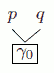
\includegraphics[scale=0.5]{5_1a}
  }
  \parbox{1.3in}{
    \centering
    $q \Gamma \gamma_0 \uplus q \Gamma' \gamma_0 =$
  }
  \parbox{0.5in}{
    \centering
    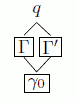
\includegraphics[scale=0.5]{5_1b}
  }
}
\par
W funkcjach, które omówimy, wszystkie dodatki do zbiorów konfiguracji, takie jak w przypadku operatora +=, domyślnie łączą stosy.
\par
Występuje szczególny przypadek związany z warunkiem stosu na początku przewidywania.
$\Gamma$ musi rozróżniać pomiędzy pustym stosem a brakiem informacji na temat stosu.
Dla przewidywania LL, początkowa symulacja stosu ATN jest bieżącym parserem stosu wywołań $\gamma_0$.
Początkowy stos jest pusty, $\gamma_0$ = [], gdy reguła decyzji wejścia jest symbolem startowym.
Przewidywanie SLL niezależne od stosu, z drugiej strony, ignoruje parser stosu wywołań i używa początkowego
stosu \# wskazując brak informacji na temat stosu.
To rozróżnienie jest ważne obliczając \textit{closure} (Funkcja 7) konfiguracji
stanowiące stan zatrzymania podmaszyny. Bez informacji stosu parsera, subparser który zwraca
z decyzji wejścia regułę A musi wziąć pod uwagę wszystkie możliwe wywołania miejsc
czyli \textit{closure} widzi konfigurację ($p'_A$,-,\#).
\par
Pusty stos [] jest traktowany podobnie jak inne węzły do przewidywania LL:
$\Gamma \uplus []$ przedstawia grafową równowartość zbioru $\{\Gamma, []\}$,
co oznacza że zarówno $\Gamma$ jak i pusty stos są dopuszczalne.
Wkładając stan p na [] mamy p[], a nie p, ponieważ pobranie p musi pozostawić symbol pustego stosu.
Dla przewidywania SLL, $\Gamma \uplus \# = \#$ dla dowolnego grafu $\Gamma$, ponieważ \# stanowi symbol
wieloznaczny i reprezentuje zbiór wszystkich stosów. Dlatego też, znak wieloznaczny zawiera wszelkie
$\Gamma$. Wkładając stan p na \# mamy p\#.

